\documentclass[../Main.tex]{subfiles}
\begin{document}
\section{Parser}
The Parser is responsible for taking a project (a folder containing a collection of code files) and extracting the methods from it. It does this by first identifying the methods inside a source file, then abstracting its content, before hashing this abstracted value. This hash is then combined with extra information concerning the method, for example the name and line number and stored in a large list. Once all files are analysed the Parser returns this list of found methods for the project. The Parser can currently parse C, C++, C\#, and Java code using srcML \cite{srcML}, while parsing Python and Javascript code using a custom parser built using ANTLR \cite{ANTLR}.\\

The class structure of the Parser can be seen in figure \cref{fig:umlparser} at the end of the documentation. The entry point for the stand-alone application is the \texttt{main} method in Main. Furthermore, the Logger class and HashData struct are used a lot throughout the entire Parser, but for clarity the arrows are not included (as they are used in most of the other classes).\\

The Parser abstracts in such a way that it can recognise type 2 code clones \cite{VUDDY, code_clones_1, code_clones_2}: meaning it removes comments and whitespaces, while abstracting variable names (including names of function calls).\\

To prevent the matching of trivial clones, any function which contain less than 50 characters (after abstraction) or six lines is excluded.\\

For hashing the Parser use the MD5 algorithm. MD5 is a very fast hash algorithm, so using MD5 as a hash algorithm allows the parser to waste little time on calculating hashes. For the implementation the "RSA Data Security, Inc. MD5 Message-Digest Algorithm" was used..


\subsection{SrcML}

\begin{figure}[h]
    \centering
    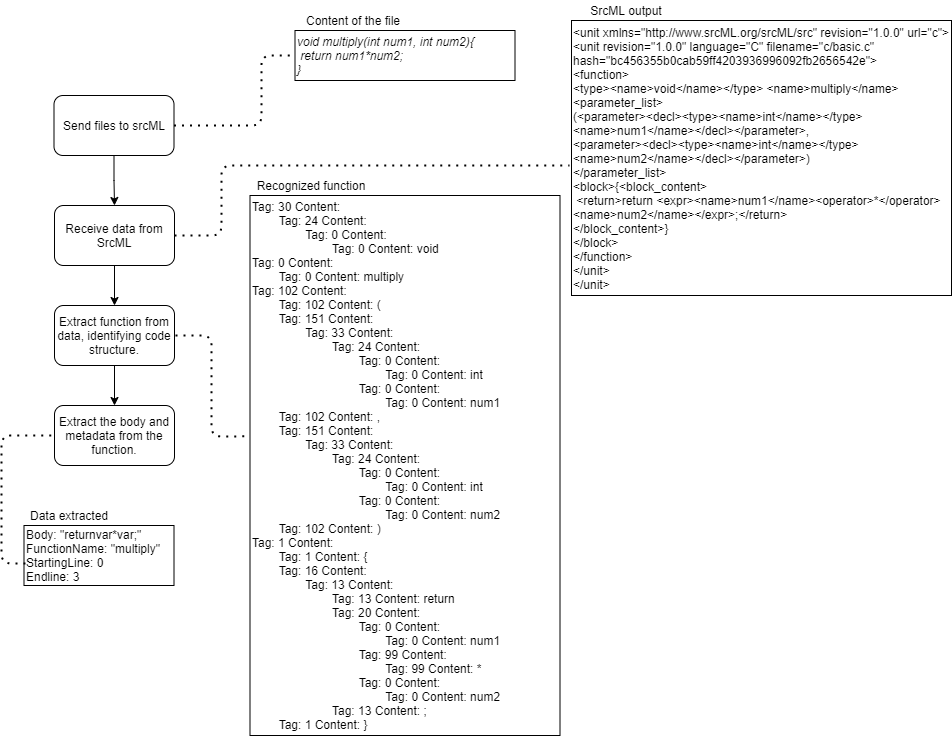
\includegraphics[width = \linewidth]{ParserSrcmlFlow.png} 
    \caption{Flow of the Parser when using srcML.}
    \label{fig:srcmlParserFlow}
\end{figure}

For C, C++, C\#, and Java files the parser uses \href{https://www.srcml.org/}{srcML} to convert source code to an XML format. This allows for easy identification of methods, as well as variables and function calls. The parser currently calls srcML using a (hidden) command line interface, since srcML can also be used as a library, it should be possible to call it directly. There have been no problems with the current approach, but there might be advantages to calling srcML directly. This calling is done by the SrcMLCaller class which starts srcML in another thread, it also creates a StringStream object which will be connected to the output of srcML and sent to the rest of the program so the output can be handled while srcML is still processing input.

SrcML is build upon ANTLR but does not use a strict parsing method, generally going through source code once assuming the format is valid. If srcML happens to encounter something that it can't understand it will simply group it under a general tag until it recognises the structure again. This makes it very fast (particularly in comparison to our own Parsers which were also made using ANTLR).

In figure \ref{fig:srcmlParserFlow} an example of the parsing using srcML is given, as well as what format data is stored between steps. The output of srcML is first parsed by the XMLParser class (XMLParser.cpp/.h) which parses the output of srcML linearly, identifying the start and end of files and methods and sending found methods to the AbstractSyntaxToHashable class. The found methods are send with the same structure received from srcML (A tree like structure where nodes identify code parts, for example a code block node, containing a number of statements, containing an assignment, containing a variable name and a value which is assigned to it, see "Recognised function" in figure \ref{fig:srcmlParserFlow}). The AbstractSyntaxToHashable then turns this tree into a single string, applying abstraction where necessary, and collecting any extra data from the method (it's name for instance), see "Data extracted" in figure \ref{fig:srcmlParserFlow}. This string is then hashed using the MD5 hashing algorithm, and saved together with any extra info (method name, file, starting/ending line).


\newpage
\subsection{Custom Parsers}
The custom parsers for Python 3 and JavaScript make use of the ANTLR4 library. Most of the ANTLR-specific information in this document will be based on the documentation from the \href{https://www.antlr.org/}{ANTLR website}. Here, ANTLR is described as follows.

\begin{quote}
    \textit{``ANTLR (ANother Tool for Language Recognition) is a powerful parser generator for reading, processing, executing, or translating structured text or binary files. It's widely used to build languages, tools, and frameworks. From a grammar, ANTLR generates a parser that can build and walk parse trees.''}
\end{quote}

An ANTLR grammar is stored with the \texttt{.g4} file extension. In essence, a grammar file is split up into a Lexer and a Parser grammar. Such a grammar consists of a declaration, followed by a list of rules. In the grammar declaration, the grammar name must be specified:\\
\begin{lstlisting}
    grammar <name>;
\end{lstlisting}\vspace{15pt}
The name of the grammar must match the name of the \texttt{.g4} file: the grammar file \texttt{X.g4} must contain the declaration \texttt{grammar X;}. Such a grammar can contain both lexer and parser rules. Similarly, a grammar with declaration \texttt{lexer grammar <name>;} can contain only lexer rules. Changing the prefix to \texttt{parser} allows only for parser rules.\\

An example of a lexer rule is the following:\\
\begin{lstlisting}
    WHILE : 'while';
\end{lstlisting}\vspace{15pt}
This simply implies that whenever we encounter the string \texttt{'while'} in the source, this should be tokenized as WHILE. Tokenizing can be seen as preprocessing the file to a list of tokens, from which a parse tree can be constructed based on the parser rules. A parser rule starts with a lowercase letter, for example:\\
\begin{lstlisting}
    file_input: (NEWLINE | stmt)* EOF;
\end{lstlisting}\vspace{15pt}
Here, the NEWLINE is defined in a lexer rule, and the stmt is defined in another parser rule. The expression \texttt{(NEWLINE | stmt)} matches is either of these rules match and the expression \texttt{(NEWLINE | stmt)* EOF} matches if there is any number of instances matching \texttt{(NEWLINE | stmt)}, followed by an end-of-file. Like this parser rule, more complex lexer rules are also possible:\\

\begin{lstlisting}
    DECIMAL_INTEGER
     : NON_ZERO_DIGIT DIGIT*
     | '0'+
     ;
\end{lstlisting}\vspace{15pt}

These rules are all examples of rules defined in the Python3 grammar from the ANTLR4 grammars on \href{https://github.com/antlr/grammars-v4}{https://github.com/antlr/grammars-v4}. We use this grammar, together with the JavaScript lexer and parser grammar from the same source, as a basis for our custom parser. We have made several small changes to these grammars to better suit our needs. These changes will be explained in detail later in this section.\\

To generate C++ code from the grammar file, we use the following bash script:
\begin{lstlisting}
java -jar antlr-4.9.2-complete.jar -visitor -Dlanguage=Cpp 
    -o generated/ Python3.g4;
\end{lstlisting}
We will now shortly look into how the parse tree is structured, to get an idea of how we can apply abstractions like those described in the previous section. We will look at a small Python3 code example to illustrate the process. This example is simply a method that doubles any input it is given:\\

\begin{lstlisting}[language=Python]
    def double(n):
        return n * 2
\end{lstlisting}
\vspace{15pt}
Using our altered version of the provided Python3 grammar, the parse tree for the code above has the following structure:\\

\begin{lstlisting}
    (file_input
      (stmt
       (compound_stmt
        (funcdef def
         (name double)
         (parameters (
          (typedargslist
           (tfpdef
            (name n))) )) :
         (funcbody
          (suite \n indent
           (stmt
            (simple_stmt
             (small_stmt
              (flow_stmt
               (return_stmt return
                (testlist
                 (test
                  (or_test
                   (and_test
                    (not_test
                     (comparison
                      (expr
                       (xor_expr
                        (and_expr
                         (shift_expr
                          (arith_expr
                           (term
                            (factor
                             (power
                              (atom_expr
                               (atom
                                (name n))))) *
                            (factor
                             (power
                              (atom_expr
                               (atom 2))))))))))))))))))) \n)) dedent))))) <EOF>)
\end{lstlisting}
\vspace{15pt}
This is a lot of data, considering the size of the input code. This is because the parser needs to specify the outer rule, before moving on to the smaller inner rules. Important things to note are that the method name \texttt{double} is contained in the first \texttt{name} tag in the bigger \texttt{funcdef} tag, and that \texttt{name} tags in the \texttt{funcbody} tag correspond to variables and function calls.\\

We can use these observations to construct an abstracted version of the method using a custom listener. This is a piece of code that can be included when walking through the parse tree, as follows:\\

\begin{lstlisting}
    antlr4::tree::ParseTreeWalker::DEFAULT.walk(&cl, t);
\end{lstlisting}
\vspace{15pt}

Here \texttt{cl} is the custom listener and \texttt{t} is the parse tree.\\

The construction of the parse tree consists of several steps. First, we tokenize the input:\\
\begin{lstlisting}
    antlr4::ANTLRInputStream input(data);
    Python3Lexer l(&input);
    antlr4::CommonTokenStream tokens(&l);
    tokens.fill();
\end{lstlisting}
\vspace{15pt}
Here, \texttt{data} is a string containing the input file. Now, we construct a parser and extract the parse tree:
\begin{lstlisting}
	Python3Parser p(&tokens);
    antlr4::tree::ParseTree* t = p.file_input();
\end{lstlisting}
\vspace{15pt}
The method \texttt{file\_input()} is generated by ANTLR, based on the parser rule for \texttt{file\_input} as seen before. This is the encapsulating rule for the entire file, so we use this to extract the entire parse tree.\\

The custom listener can overwrite methods such as \texttt{enterFuncdef} and \texttt{exitFuncdef}, which can be found in the base listener generated by ANTLR. Like the name suggests, these methods are called upon entering and exiting a \texttt{funcdef} tag. We override several of these functions to extract and abstract method bodies. Since function definitions can be nested, we store all important data in stacks: starting line numbers, function names and function bodies. Furthermore, we also store a stack of so-called \texttt{TokenStreamRewriter} objects. These are used to dynamically store changes to the parse tree. The stored changes are only applied when we retrieve the abstracted method as a string, which is why we chose to use a \texttt{TokenStreamRewriter} per method, instead of a single \texttt{TokenStreamRewriter} for the entire file. This massively speeds up the program, since the changes stored in processed methods can be discarded after the method has been abstracted, by deleting the \texttt{TokenStreamRewriter} object.\\

The custom listener for Python 3 overrides the following methods:
\begin{itemize}
    \item \texttt{enterFuncdef}: Called when a new method definition is entered. We prepare for computing the abstracted hash-data of this method by pushing a new \texttt{TokenStreamRewriter}, an empty function name and function body and the current line as a starting line to their respective stacks.
    \item \texttt{exitFuncdef}: Called when a method definition is exited. We pop all method data from the stacks and store the current line as the ending line. Check if an abstracted method longer than $6$ lines and $50$ characters and if so, hash the method body with MD5 and store all data in the \texttt{output} vector.\\
    
    If this method definition was given in another method definition, we abstract the inner method to the empty string. This is because a method defined in another method could just as well have been defined outside of the outer method.
    \item \texttt{enterFuncbody}: Called when a method body is entered. Store this by setting the \texttt{inFunction} boolean to \texttt{true}. This is used to only abstract terms inside the method body.
    \item \texttt{exitFuncbody}: Called when a method body is exited. Here, we extract the text of the entire \texttt{funcbody} tag from the top \texttt{TokenStreamRewriter}, which was used to abstract the current method body:
    \begin{lstlisting}
functionBodies.top() = tsrs.top()->getText(ctx->getSourceInterval());
    \end{lstlisting}
    \item \texttt{enterName}: Called when an unknown name is entered. A name is a string which is used in an expression, but is not a function call. In general, this consists mostly of variables. We thus abstract all names in a function body to "var":
    \begin{lstlisting}
tsrs.top()->replace(ctx->start, "var");
    \end{lstlisting}

    Like we saw above, the name of the method is the first name tag in a funcdef tag. We also check this in this method.
    \item \texttt{enterFunccallname}: This is similar to the \texttt{enterName} method, but the funccallname tag is solely for function calls. These are abstracted to the string "funccall":
    \begin{lstlisting}
tsrs.top()->replace(ctx->start, "funccall");
    \end{lstlisting}
    \item \texttt{enterExpr\_stmt\_single}: Called when an expression with only a single statement is entered. We store this by setting the \texttt{inSingleStatement} boolean to \texttt{true}.
    \item \texttt{exitExpr\_stmt\_single}: Called when an expression with only a single statement is exited. We store this by setting the \texttt{inSingleStatement} boolean to \texttt{false}.
    \item \texttt{enterString}: Called when a string is entered. This is a string in Python, so \texttt{'abc'} or \texttt{"abc"}, or even a multiline string (\texttt{'''abc'''} or \texttt{"""abc"""}). Generally, we do not abstract these strings, and simply keep them as-is. However, an expression solely consisting of a single string is ignored by Python. This behaviour is often used to create multiline comments. Since these have no impact on the functionality of the method, we want to ignore it. Therefore, we replace any string by the empty string if the \texttt{inSingleStatement} is set to \texttt{true}.
\end{itemize}


Using our Python3 parser, the \texttt{double} method is abstracted as follows:\\
\begin{lstlisting}
    indentreturnvar*2
    dedent
\end{lstlisting}
\vspace{15pt}
This is then hashed with MD5 and returned together with the starting and ending line of the method (including header) and its name, which in this case is \texttt{double}.\\

The second custom parser we created is the JavaScript parser. This is based on the same ideas as the Python parser, and is implemented in a similar way. A change in how the JavaScript parser abstracts methods, is that function calls are also abstracted as "var". This is possible, since all function calls in JavaScript are immediately followed by an opening bracket and variables are never followed by an opening bracket. The fragment "var(" thus uniquely identifies a function call. Like mentioned before, the JavaScript grammar is split up into a lexer and parser grammar, but the code can be generated in the same way, by simply generating the lexer code, followed by generating the parser code with the following bash script:
\begin{lstlisting}
java -jar antlr-4.9.2-complete.jar -visitor -Dlanguage=Cpp 
    -o generated/ JavaScriptLexer.g4;
java -jar antlr-4.9.2-complete.jar -visitor -Dlanguage=Cpp 
    -o generated/ JavaScriptParser.g4;
\end{lstlisting}

The general structure of the JavaScript custom listener is the same, but we override different methods:
\begin{itemize}
    \item \texttt{enterAnonymousFunctionDecl}: Called when an anonymous function declaration is entered. JavaScript has different types of functions, including anonymous functions. These are functions without a name. Like with the Python 3 parser, we push a new \texttt{TokenStreamRewriter}, an empty function name and function body and the current line as a starting line to their respective stacks. Furthermore, we set the \texttt{inNonAbsFuncDef} boolean to \texttt{false}, indicating that we are in an anonymous function definition. This is mainly used to indicate that we do not need to bother with finding a function name, since there is none.
    \item \texttt{enterFunctionDeclaration}: Called when a non-anonymous function declaration is entered. This mostly does the same as \texttt{enterAnonymousFunctionDecl}, but it sets the \texttt{inNonAbsFuncDef} boolean to \texttt{true}.
    \item \texttt{exitAnonymousFunctionDecl}: Called when an anonymous function declaration is exited. We do the same as with the Python 3 parser and pop all stacks, get the current line as ending line and store the MD5 hash of the method if it is longer than $6$ lines and $50$ characters. An anonymous function is mostly used as a variable in an outer method, so we abstract the entire method to "var" after storing the abstracted method.\\
    \item \texttt{exitFunctionDeclaration}: Called when a non-anonymous function declaration is exited. This mostly does the same as \texttt{exitAnonymousFunctionDecl}, but it abstracts the entire method to the empty string after storing the abstracted method. By the same reasoning as in the Python 3 parser, a non-abstract method could also have been declared outside of the current method.
    \item \texttt{enterParseFunctionBody}: Called when the body of a method declaration is entered. This implies that we exited the method header, so we set the \texttt{inNonAbsFuncDef} boolean to \texttt{false}.
    \item \texttt{exitParseFunctionBody}: Called when the body of a method declaration is exited. Here, we store the abstracted function body in exactly the same way as in the Python 3 parser:
    \begin{lstlisting}
functionBodies.top() = tsrs.top()->getText(ctx->getSourceInterval());
    \end{lstlisting}
    \item \texttt{enterIdentifier}: Called when an identifier is entered. This can be both a variable or function call, but in both cases, we abstract this to "var". The single exception to this is the extraction of the method name. Similar to the Python 3 parser, this is the first \texttt{identifier} tag in the \texttt{functionDeclaration} block. Therefore, if \texttt{inNonAbsFuncDef} is \texttt{true} and the function name is not yet known, we store the current \texttt{identifier}:
    \begin{lstlisting}
if (inNonAbsFuncDef && functionNames.top() == "")
	{
		functionNames.top() = ctx->start->getText();
	}
    \end{lstlisting}
\end{itemize}

To improve the custom parsers, we first studied the parse tree of a given piece of source code and looked for potentially interesting patterns, such as the strings in single expressions as a comment in Python 3. We then changed the grammar to create a specific rule (tag) for this case and regenerated the generated C++ code. The custom listener was then changed to include this new tag, and handle it as we desired. A potential improvement would definitely be to write a grammar from sratch, with fewer rules. This is probably possible, since we do not use all of the intricacies of a language and apply quite a basic abstraction. This has the potential to greatly speed up the parser, depending on how minimal the resulting grammar is.\\

The general structure of the custom parsers can be seen in the UML diagram in Appendix A. In essence, both custom parsers are subclasses of the \texttt{LanguageBase} class, as defined in LanguageBase.h. The main method this class describes is the \texttt{parseData} method. This parses an entire source file to a vector of HashData structs, containing all information required of a hashed method. It also contains the \texttt{ClearCache} method, required for garbage collection purposes. These two methods are implemented in the \texttt{Python3AntlrImplementation} and \texttt{JavaScriptAntlrImplementation} subclasses (as the names suggest, one class for the Python 3 parser and another for the JavaScript parser). These classes handle the construction and traversing of parse trees, a procedure described above. While traversing the parse tree, they make use of the custom listeners defined in the \texttt{CustomPython3Listener} and \texttt{CustomJavaScriptListener} classes. These are subclasses of the ANTLR-generated \texttt{Python3BaseListener} and \texttt{JavaScriptParserBaseListener} classes and contain the method overrides as listed above.
\end{document}